\subsection{Chris Pham}
\subsubsection{Week 1}
This first week of classes for the three of us was mostly planning on what to exactly doing for the next 10 weeks and what exactly our working times are.
We planned for Tuesdays, Thursdays, and Saturdays because that's when Ken is supposed to be down and everyone seems to be free on those days.
Another thing that did come up was that the expectation that we should go to the OSU Robotics Club's Mars Rover Meetings on Saturday at 12 in the afternoon.
Another bonus of Saturday's is that that is when the team has working hours and we can interact with the people creating the systems on the rover side.
After deciding our times, we decided on who should do what task using our Asana and dictated by the club and our client.
It was decided that I would be doing Mapping and the others doing video and connection statuses.
\\
I was first prototyping using the Google Maps Static API and Python 2.7 to grab the tile at the given GPS location.
It worked, but I ended up thinking about how to stitch this object correctly.
I was also contemplating zooming in on the image instead of using stitching to remove complexity.
I do not have my code now from testing out the API because I reformatted this computer completely to install the requirements for the project, Ubuntu 16.04 and more importantly ROS.
\subsubsection{Week 2}
On Saturday, I started working on trying to search how to stitch images using Google Images.
I was told that last year they used this class package called GooMPy that took care of that for them and I spent my time looking at this code and trying to understand what it does.
We also took a group photo and I was introduced to the software team of the Rover.
It turned out they're mostly Freshman and they did not finish their Python reviews yet, so they could not start on the rover software that we need to interact with.
\\
On Tuesday, we met up in our club room and did some basic things with Qt Designer so we would be caught up on designing that.
I had some questions about some things like the API calling limit we have for Google Maps, and it turns out we will almost never hit the API limit.
Another thing was multi-threaded performance because how this file worked was that it did a bunch of Google Maps calls and then merged them with PIL (Python Image Library) and this looked doable to multi-thread.
However, one issue we have is the effect of Qt's QThreads and the multi-threading process for Python playing nicely with each other.
After talking about that, I then made created a branch in git and then built my files based upon GooMPy and made it more class based so it makes more sense for grouping and private variables.
The troubles with the structured format of the old file makes it hard to understand with the lack of comments and weird structures that is not expected in Python. 
All progress during this week was during January 18, 2018:\\
\begin{center}
\begin{tabular}{l l l l}	\textbf{Detail} & \textbf{Author} & \textbf{Date} &\textbf{Description}\\\hline
\href{https://github.com/OSURoboticsClub/Rover_2017_2018/commit/bb8ed586e278eaa18b1861a0949afa53a743c876}{bb8ed58} & Chris Pham & 2018-01-18 10:37:41 -0800 &Make Mapping Core (mapping.py)\\\hline
\href{https://github.com/OSURoboticsClub/Rover_2017_2018/commit/47942ffd1dcc2b3a1e29776d00a005f5a4247ea3}{47942ff} & Chris Pham & 2018-01-18 10:40:47 -0800 &Added Imports\\\hline
\href{https://github.com/OSURoboticsClub/Rover_2017_2018/commit/c8c8f857cd2de7d01a5c790a22ac643a6b962436}{c8c8f85} & Chris Pham & 2018-01-18 10:47:56 -0800 &Add Constants\\\hline
\href{https://github.com/OSURoboticsClub/Rover_2017_2018/commit/a9f36af40d4c3a00bb2336852d0db329f3b5905e}{a9f36af} & Chris Pham & 2018-01-18 10:53:39 -0800 &Read key from file\\\hline
\href{https://github.com/OSURoboticsClub/Rover_2017_2018/commit/7e593097eab330b71a54b56251a1bea11e31a72c}{7e59309} & Chris Pham & 2018-01-18 10:55:42 -0800 &Made apikey file, and fixed open error\\\hline
\href{https://github.com/OSURoboticsClub/Rover_2017_2018/commit/b82a39d3bf666abd8ed38839d6c5730b09e6ad04}{b82a39d} & Chris Pham & 2018-01-18 10:58:24 -0800 &fixed fp naming conventions\\\hline
\href{https://github.com/OSURoboticsClub/Rover_2017_2018/commit/3570c4b5735bc2dbdf39bb5f52d34ccaa5bbee7e}{3570c4b} & Chris Pham & 2018-01-18 11:09:09 -0800 &write file intro\\\hline
\href{https://github.com/OSURoboticsClub/Rover_2017_2018/commit/a9bf793bfc0db615d7d62bef7ac1d56f81c38d6c}{a9bf793} & Chris Pham & 2018-01-18 11:21:05 -0800 &add gmaps obj and init\\\hline
\href{https://github.com/OSURoboticsClub/Rover_2017_2018/commit/c2bb5f6d31e6457d59e207c5f87edeeb2ac50e11}{c2bb5f6} & Chris Pham & 2018-01-18 12:14:06 -0800 &Added pixel\_to\_degrees helper\\\hline
\href{https://github.com/OSURoboticsClub/Rover_2017_2018/commit/f203cee53e0a60c4dc8eed40dfae0a07e4649e59}{f203cee} & Chris Pham & 2018-01-18 12:24:01 -0800 &rebuild Google Maps API link\\\hline
\href{https://github.com/OSURoboticsClub/Rover_2017_2018/commit/d09dbb1a02bc8883bc16e68aa8de74ee1b6ecfe6}{d09dbb1} & Chris Pham & 2018-01-18 12:43:03 -0800 &Addded \_grab\_tile helper\\\hline
\href{https://github.com/OSURoboticsClub/Rover_2017_2018/commit/16f76fad49699b346e15c0fdcfc2edcb814a0123}{16f76fa} & Chris Pham & 2018-01-18 13:00:53 -0800 &added \_pixels\_to\_lon helper\\\hline
\href{https://github.com/OSURoboticsClub/Rover_2017_2018/commit/b7348ee897a3bbff349d2d04d7c2084bc60c46f0}{b7348ee} & Chris Pham & 2018-01-18 13:07:21 -0800 &Fix self in pixel\_to\_lon helper\\\hline
\href{https://github.com/OSURoboticsClub/Rover_2017_2018/commit/400410cea4af92cb25fd1f686809f320c9cc102c}{400410c} & Chris Pham & 2018-01-18 13:21:38 -0800 &Added \_pixels\_to\_lat\\\hline
\href{https://github.com/OSURoboticsClub/Rover_2017_2018/commit/d2f4fc38fecf903ed35d731dafe566709707601c}{d2f4fc3} & Chris Pham & 2018-01-18 13:23:48 -0800 &Add gitignore for API key\\\hline
\href{https://github.com/OSURoboticsClub/Rover_2017_2018/commit/b319118e1d32c8d655afe7a6cd084916d16f8db3}{b319118} & Chris Pham & 2018-01-18 13:26:03 -0800 &remove key\\\hline
\end{tabular}
\end{center}
\subsubsection{Week 3}
During the meeting on Saturday, I was informed that there is a API key and signature that I should use so I don't get throttled nor limited on calls.
I was finishing up some of my helper functions for my class object and then fixed my code to fit PEP8 conventions.
Then to implement my code, I made a new file called sign.py to take in a string and then return me the correct signature to append to the string for Google to accept.
Once that was done, I built a testing script to call the object and then save the big image somewhere on my computer.
Turns out my laptop hates that and I froze my computer for 20 minutes and once that was done, I edited the .gitignore to ignore the .jpg files I was downloading from the API.
\\
On Thursday, I was trying to get my zooming to work correctly on this image, but I can't do it from the API and I would have to do it from Qt or from OpenGL.
I also made a smaller display image to display it onto the display space on the GUI and for my computer to run.
\begin{center}
\begin{tabular}{l l l l}
\textbf{Detail} & \textbf{Author} & \textbf{Date} &\textbf{Description}\\\hline
\href{https://github.com/OSURoboticsClub/Rover_2017_2018/commit/995386ee89319296165900b1466b6cfc5cf060d5}{995386e} & Chris Pham & 2018-01-20 13:06:28 -0800 &Made pixels\_to\_meters helper\\\hline
\href{https://github.com/OSURoboticsClub/Rover_2017_2018/commit/fee5b5537bbdb496791f7b7f323aae6995844afc}{fee5b55} & Chris Pham & 2018-01-20 13:24:32 -0800 &Added logic for num\_sqares\\\hline
\href{https://github.com/OSURoboticsClub/Rover_2017_2018/commit/3565e7b57f1f19a81b9b34b88a8c9ef527e7c7d6}{3565e7b} & Chris Pham & 2018-01-20 13:43:47 -0800 &Rebuild grab\_tile\\\hline
\href{https://github.com/OSURoboticsClub/Rover_2017_2018/commit/e955442131978ffd1d24aa6ced9ff2c9f899ed59}{e955442} & Chris Pham & 2018-01-20 13:57:11 -0800 &Fixed to fit PEP\\\hline
\href{https://github.com/OSURoboticsClub/Rover_2017_2018/commit/332c751758c837cb52b3a9008ba830c5755fbf76}{332c751} & Chris Pham & 2018-01-20 14:14:44 -0800 &Append signature\\\hline
\href{https://github.com/OSURoboticsClub/Rover_2017_2018/commit/a0601abb8db35bf4a7ebcdba81f702814c73fdf2}{a0601ab} & Chris Pham & 2018-01-20 16:32:58 -0800 &Add testing file with updated gitignore for jpgs\\\hline
\href{https://github.com/OSURoboticsClub/Rover_2017_2018/commit/1c16cb48a1faec2e8dc157748d0f870d1253fde7}{1c16cb4} & Chris Pham & 2018-01-25 10:49:36 -0800 &Creates Big Image\\\hline
\href{https://github.com/OSURoboticsClub/Rover_2017_2018/commit/b12f8fc986912d75d018e8da9912eaa1c93b9e4b}{b12f8fc} & Chris Pham & 2018-01-25 15:01:35 -0800 &Working updates and fetching, starting on zoom functionality\\\hline
\end{tabular}
\end{center}
\subsubsection{Week 4}
This week, I had a bunch of troubles trying to get most of my stuff working correctly.
One big issue with my code was the latitude and longitude values to pixel coordinates. For some reason my values would be pointing to the wrong locations.
From the research I did about this issue, I can explain better why these equations are used at least.
I spent around 4 hours working on this and I had to leave to do something else on the side.
\\
I was thinking it could be the skew from the center of the map towards the outsides compared to just getting the outside values at the start.
I tried to get the boundaries when generating map and then cutting the value in half to get the approximate centering.
That did not work at all and I just gave up on it for a bit and went ahead and tried to program something else like putting icons on the map correctly.
Somehow, when I copied the code from the previous function, and then used it, it provided the correct locations and I was really confused.
Then I used the function that I just made and used that to center my map to see if that worked and it did.
Once I got that part working, I then made some way of adding icons to the image to quickly prototype my way-point system.
Here are some examples of my code via images, before and after:
\begin{figure}[ht!]
\begin{minipage}[t]{.45\linewidth}\centering
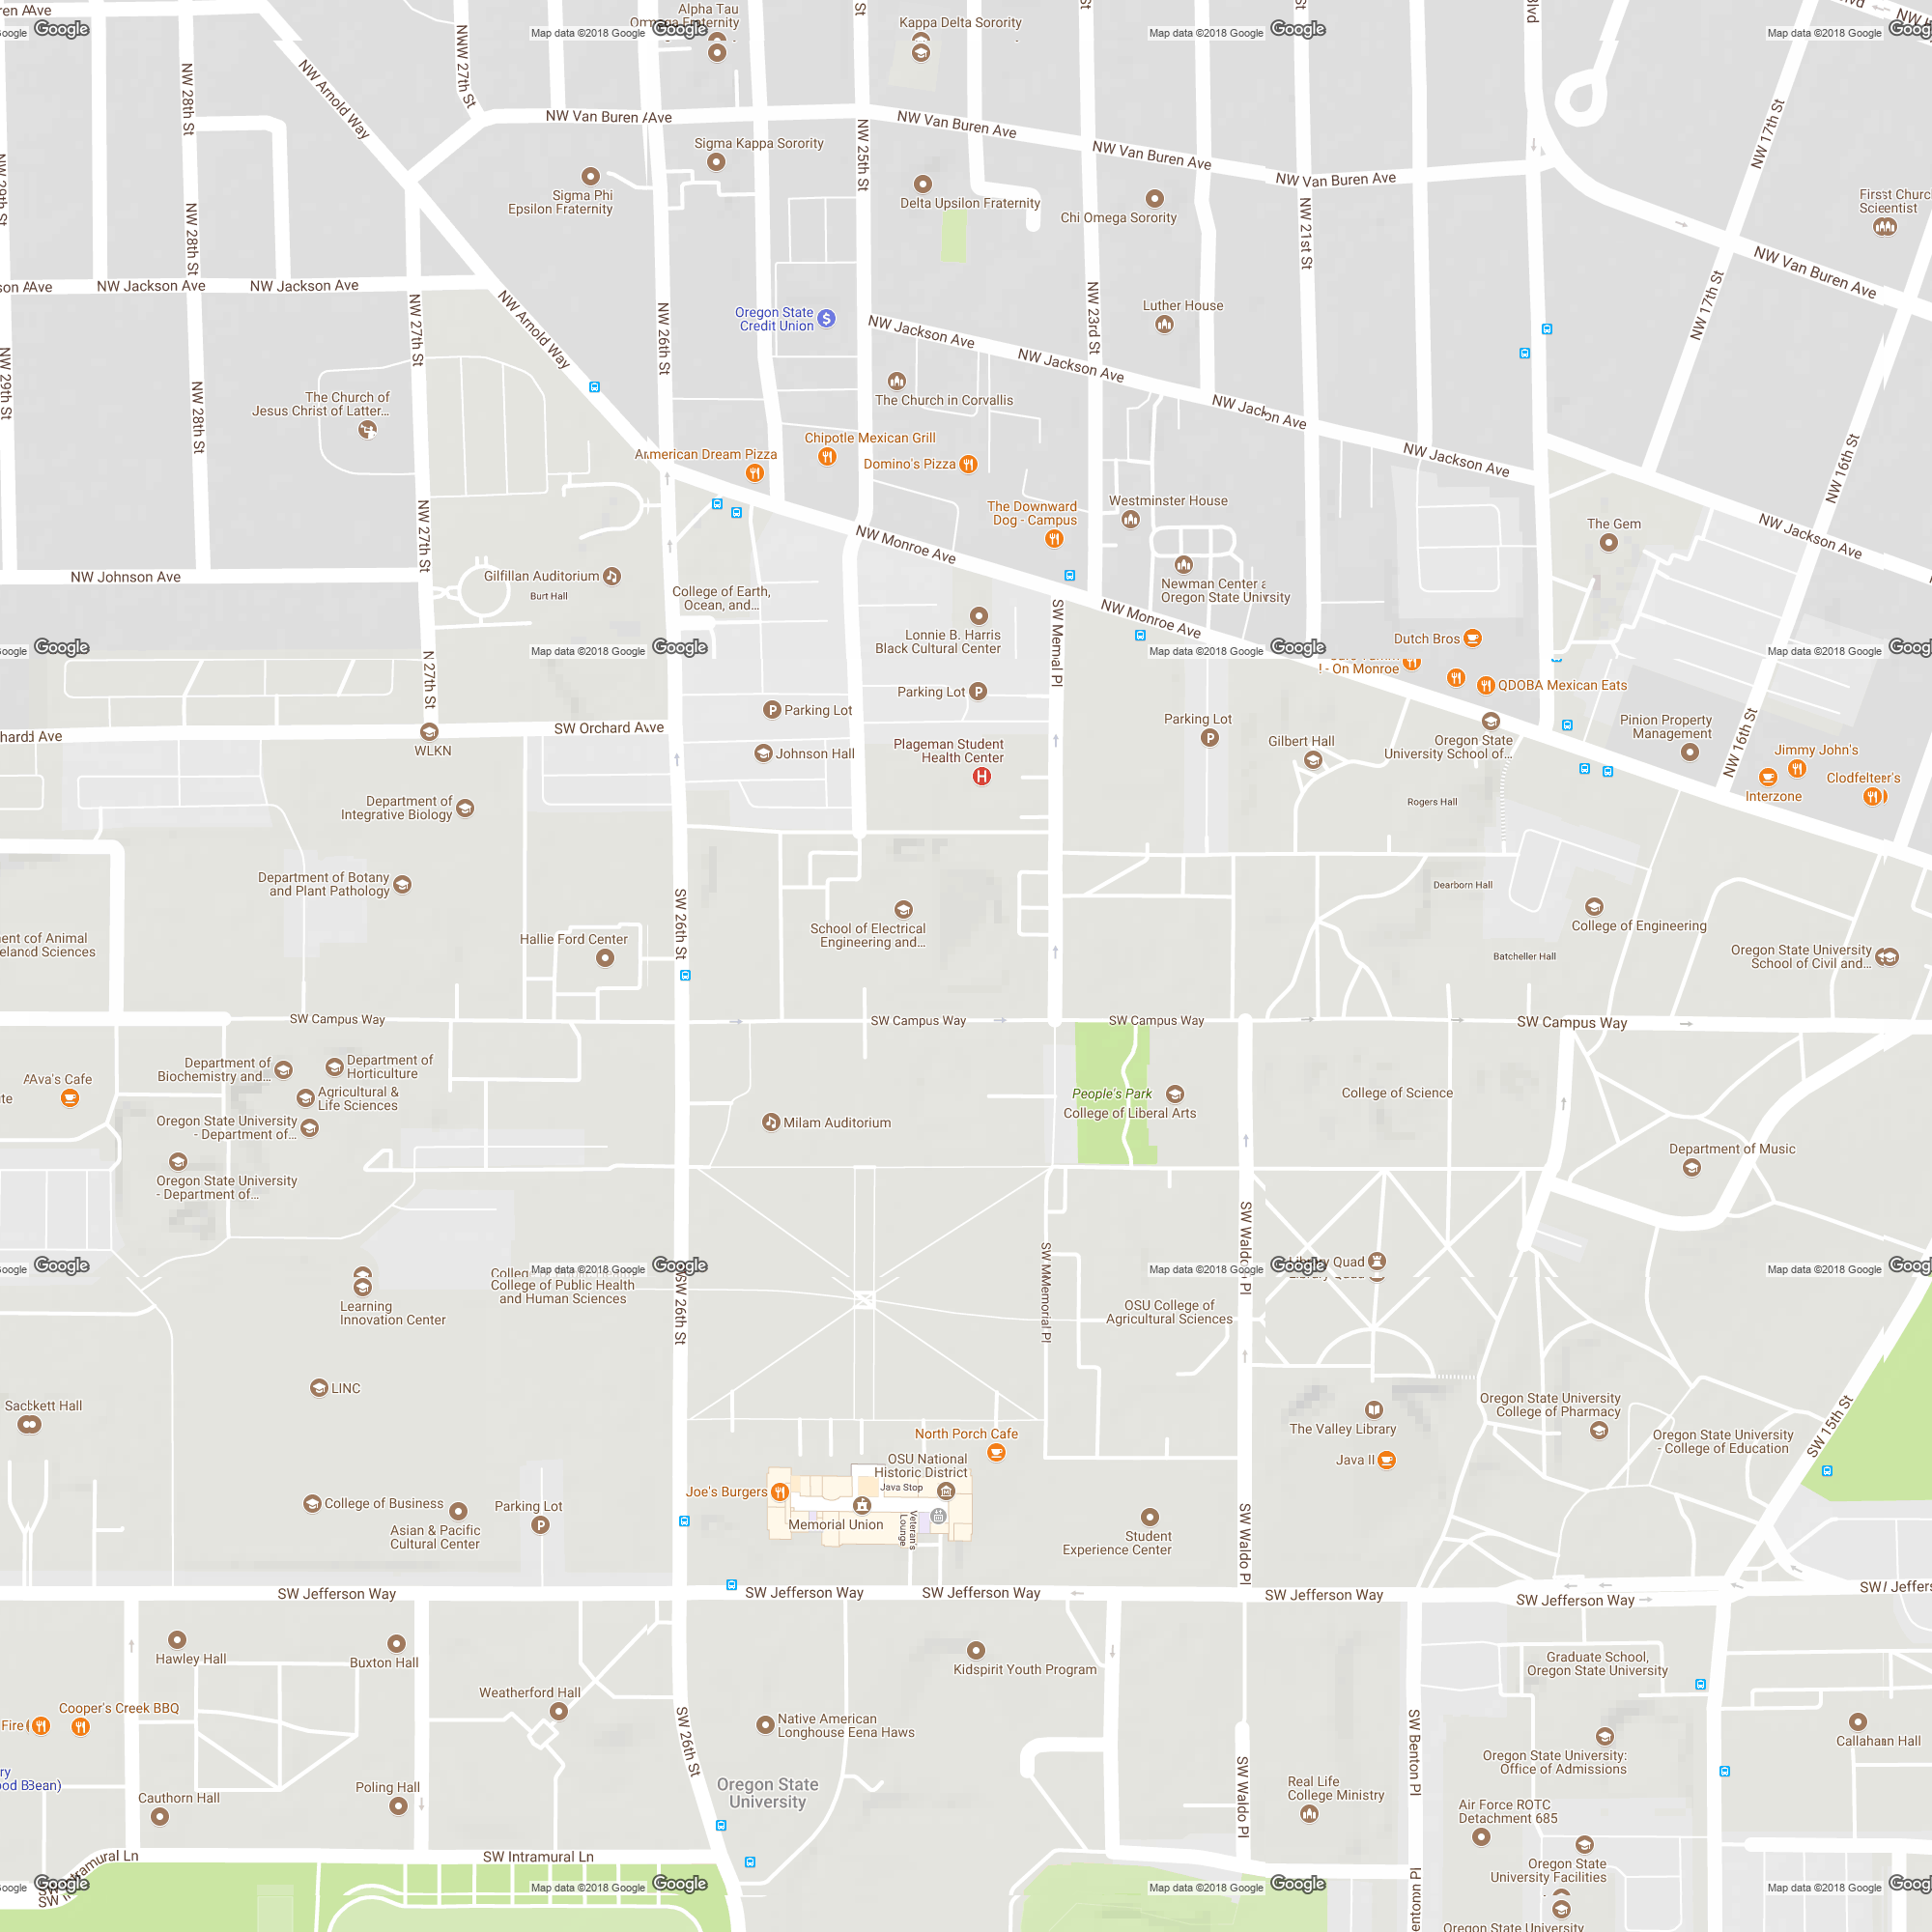
\includegraphics[width=\linewidth]{figures/unzoomed}
\caption{Before, Centered at Kelly}
\end{minipage}\hfill
\begin{minipage}[t]{.45\linewidth}\centering
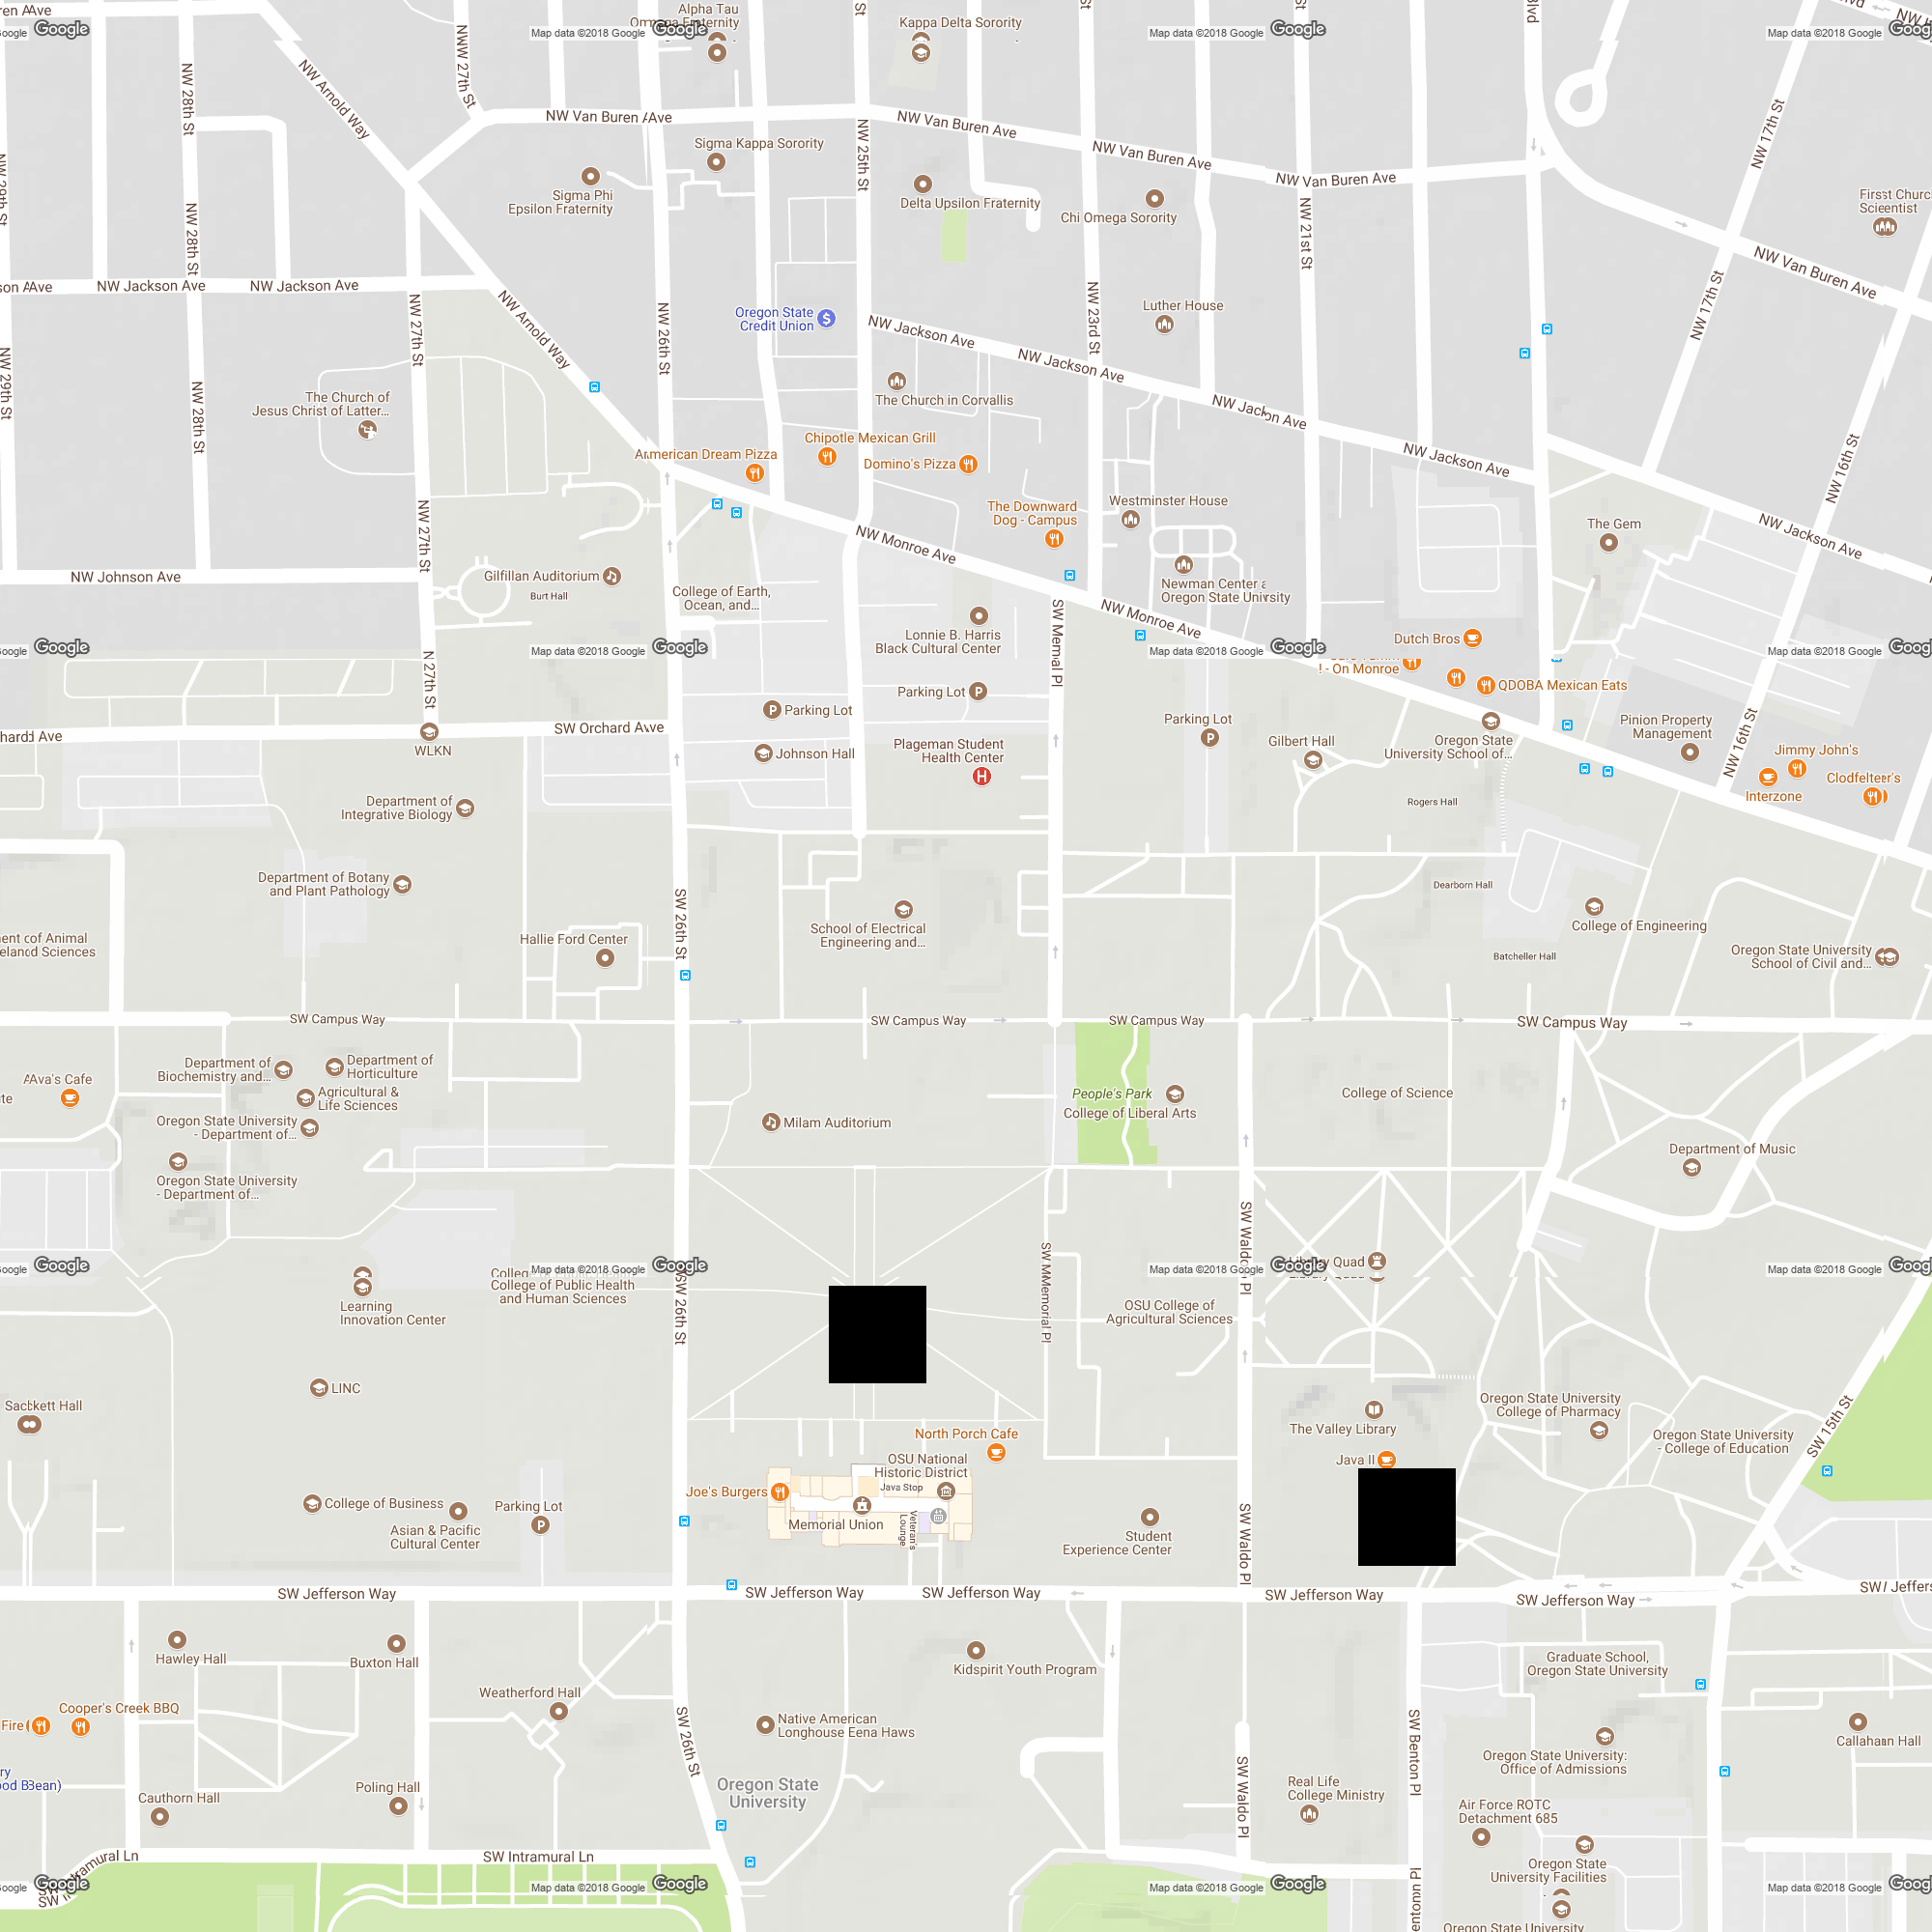
\includegraphics[width=\linewidth]{figures/centered}
\caption{After, Centered at Kelly and points at MU and Valley}
\end{minipage}
\end{figure}
\newline
One of the next issues I thought about was trying to reduce computation time and I was thinking of using a way-point later to control and manage any drawing on the screen.
I can make a transparent layer/image with alpha levels with icons I can inject via PIL that I can draw each time instead of using disk time to get the images again
That can be done using Qt I think, or even PIL can do it, but it might take a hit on computation times.
\begin{center}
\begin{tabular}{l l l l}	\textbf{Detail} & \textbf{Author} & \textbf{Date} &\textbf{Description}\\\hline
\href{https://github.com/OSURoboticsClub/Rover_2017_2018/commit/3ed2c5977e41dc8f4baee7b10d7c3114793e29d7}{3ed2c59} & Chris Pham & 2018-02-01 19:25:54 -0800 &created and fixed centering\\\hline
\href{https://github.com/OSURoboticsClub/Rover_2017_2018/commit/5f12d8074f8fcfb799f6ac3493cb39081bb7f7c3}{5f12d80} & Chris Pham & 2018-02-01 19:55:57 -0800 &starting on map updatiing\\\hline
\href{https://github.com/OSURoboticsClub/Rover_2017_2018/commit/75adf70d5bfba0e4b7b48bf7cefbc88feb68f4de}{75adf70} & Chris Pham & 2018-02-02 11:30:16 -0800 &define \_\_str\_\_\\\hline
\href{https://github.com/OSURoboticsClub/Rover_2017_2018/commit/d012360da50b074efb9a1cc1f7c1e0dacda207e7}{d012360} & Chris Pham & 2018-02-02 13:11:06 -0800 &remove prints\\\hline
\hline\end{tabular}
\end{center}
\subsubsection{Week 5}
This week was building and refactoring my object class so it had a helper class to do work for it too.
I rearranged it because I needed to use some of those function myself for building the way-point overlay system I going to implement for my system.
On Saturday, I merged my branch into the Master, but that took a bit of time because I had to rebase my branch into fitting the current master branch.
Once it was rebased to fit the master branch, I then had to do some 'git mv' to move some files around go the correct locations.
Once that was finished, I could finish my pull request and I could go on with some other tasks.
I started commenting and documenting my progress using docstrings and then applying PEP8 standard for the rest of my code, which meant that I needed to decrease the amount of characters were on a line most of the time.
After finishing up all of that, I started on making the coordinator between the class and the QObject that I needed to use to get Qt to work correctly with this object.
\begin{center}
\begin{tabular}{l l l l}\textbf{Detail} & \textbf{Author} & \textbf{Date} & \textbf{Description}\\\hline
\href{https://github.com/OSURoboticsClub/Rover_2017_2018/commit/15154f912ff4204e8a3bcf48299592d1fb8bc2ca}{15154f9} & Chris Pham & 2018-02-03 12:49:43 -0800 &Merge branch 'Mapping\_Core' of https://github.com/OSURoboticsClub/Rover\_2017\_2018 into Mapping\_Core\\\hline
\href{https://github.com/OSURoboticsClub/Rover_2017_2018/commit/07534f8487ba8a04d63e73c22385158479c3c6cc}{07534f8} & Chris Pham & 2018-02-03 13:45:51 -0800 &Starting of mapping class refactor\\\hline
\href{https://github.com/OSURoboticsClub/Rover_2017_2018/commit/06c605ebd5780e65f1f7ad077ef5cf7a136d2a18}{06c605e} & Chris Pham & 2018-02-03 13:46:46 -0800 &remove idea file\\\hline
\href{https://github.com/OSURoboticsClub/Rover_2017_2018/commit/e65d4e5067d4b3f9b1223a57f7666131e2c2cf6f}{e65d4e5} & Chris Pham & 2018-02-03 13:50:32 -0800 &Move new\_image function to helper\\\hline
\href{https://github.com/OSURoboticsClub/Rover_2017_2018/commit/37303e3a95020e41aadea474e2d6e95c543f5af0}{37303e3} & Chris Pham & 2018-02-03 13:53:21 -0800 &Moved fast\_round to helper\\\hline
\href{https://github.com/OSURoboticsClub/Rover_2017_2018/commit/0cbd593380d86ca3d479b7e40167273641c8c04d}{0cbd593} & Chris Pham & 2018-02-03 13:56:15 -0800 &Add pixels\_to\_degrees to helper\\\hline
\href{https://github.com/OSURoboticsClub/Rover_2017_2018/commit/10c9dc8451a582e67e8475e2bf161054191f1d02}{10c9dc8} & Chris Pham & 2018-02-03 14:02:23 -0800 &Make static functions and self reference for helper\\\hline
\href{https://github.com/OSURoboticsClub/Rover_2017_2018/commit/4a66dbc0b5954672d4377a1c9e07c53ccd1d7323}{4a66dbc} & Chris Pham & 2018-02-03 14:06:46 -0800 &Moved pixels\_to\_meters to Helper\\\hline
\href{https://github.com/OSURoboticsClub/Rover_2017_2018/commit/d17aaf5ef8343be017032c46fa391b9b27470bc2}{d17aaf5} & Chris Pham & 2018-02-03 14:37:43 -0800 &Added Docstrings for mapping.py\\\hline
\href{https://github.com/OSURoboticsClub/Rover_2017_2018/commit/b402cd12d3ab294d280cddf85c28ac263f62ce91}{b402cd1} & Chris Pham & 2018-02-03 14:40:46 -0800 &created docstrings for maphelper\\\hline
\href{https://github.com/OSURoboticsClub/Rover_2017_2018/commit/ad51c3d7940eb1c5baa8f4ac0b72fe115c7eb776}{ad51c3d} & Chris Pham & 2018-02-03 14:51:32 -0800 &Finished move\_latlon function\\\hline
\href{https://github.com/OSURoboticsClub/Rover_2017_2018/commit/31ad2185cb708d66cdb29dc23597a8c241622b4f}{31ad218} & Chris Pham & 2018-02-03 14:52:20 -0800 &Comment out waypoints\\\hline
\href{https://github.com/OSURoboticsClub/Rover_2017_2018/commit/23f3554af37f18f17b1ad9c79378f5fc185ebf1a}{23f3554} & Chris Pham & 2018-02-03 15:28:45 -0800 &complying with PEP8 standard\\\hline
\href{https://github.com/OSURoboticsClub/Rover_2017_2018/commit/89e7739f54adcf9317261f4741d1860d9c41a838}{89e7739} & Chris Pham & 2018-02-08 12:58:45 -0800 &Start of RoverMapCoordinator\\\hline
\href{https://github.com/OSURoboticsClub/Rover_2017_2018/commit/33694343176eaedff94334df4083b831ce1bc006}{3369434} & Chris Pham & 2018-02-08 13:33:32 -0800 &Changed file names and started initer for MapCoordinator\\\hline
\href{https://github.com/OSURoboticsClub/Rover_2017_2018/commit/f4d6835e85304f1dd43cea14ac4eb17587b14606}{f4d6835} & Chris Pham & 2018-02-08 13:50:12 -0800 &create label for left xml for map location, and remove \_get\_map.\\\hline
\href{https://github.com/OSURoboticsClub/Rover_2017_2018/commit/4455e5769389aa18ea396a3981cf3a3b989c6271}{4455e57} & Chris Pham & 2018-02-08 13:57:49 -0800 &fixed wrong size references\\\hline
\href{https://github.com/OSURoboticsClub/Rover_2017_2018/commit/cdfc76789173155e7f6fdc8d27137149e6f41fc6}{cdfc767} & Chris Pham & 2018-02-08 14:02:43 -0800 &Corrcted bool and created the thread for the main class\\\hline
\href{https://github.com/OSURoboticsClub/Rover_2017_2018/commit/bb3b47977b1818ff9d45c6144d134e6a34a7d316}{bb3b479} & Chris Pham & 2018-02-08 14:06:12 -0800 &Moved file to software/ground\_station\\\hline
\href{https://github.com/OSURoboticsClub/Rover_2017_2018/commit/e9f03deaa25624aeec6509c72e782cc801fef521}{e9f03de} & Chris Pham & 2018-02-08 14:08:26 -0800 &Merge pull request \#9 from OSURoboticsClub/Mapping\_Core\\\hline
\href{https://github.com/OSURoboticsClub/Rover_2017_2018/commit/f71bcba2b080bbc51f9d5eda2f2ae3010d332f68}{f71bcba} & Chris Pham & 2018-02-08 14:13:53 -0800 &Change the include to correct path and remove test file\\\hline
\href{https://github.com/OSURoboticsClub/Rover_2017_2018/commit/fe53c5d5a73ac253acaef11fef448995f519cca8}{fe53c5d} & Chris Pham & 2018-02-08 14:36:12 -0800 &added init for mapping\\\hline
\href{https://github.com/OSURoboticsClub/Rover_2017_2018/commit/79325aefdf731ab4fcadc9dee58e3359e6c3b289}{79325ae} & Chris Pham & 2018-02-08 14:39:46 -0800 &Added parenthesis\\\hline
\href{https://github.com/OSURoboticsClub/Rover_2017_2018/commit/345c75886dfaf76865e56aedc130ec83f9dd8352}{345c758} & Chris Pham & 2018-02-08 14:40:48 -0800 &remove bang\\\hline
\href{https://github.com/OSURoboticsClub/Rover_2017_2018/commit/8b903d1299d30611ca22aaebc5267e874de4c004}{8b903d1} & Chris Pham & 2018-02-08 14:44:20 -0800 &changed import calls and another bang\\\hline
\href{https://github.com/OSURoboticsClub/Rover_2017_2018/commit/e64c42c45fa51556a9e4e2fba3f2e0450f75a134}{e64c42c} & Chris Pham & 2018-02-08 14:51:35 -0800 &correct super \_\_init\_\_ for map coord\\\hline
\href{https://github.com/OSURoboticsClub/Rover_2017_2018/commit/cba5bc9b39738a42df87b09cea98ffc9599b9617}{cba5bc9} & Chris Pham & 2018-02-08 14:59:56 -0800 &Create setup\_signals for Map Coords\\\hline
\href{https://github.com/OSURoboticsClub/Rover_2017_2018/commit/c50675b30154dfe9d87e9b7e2cb8d02caafc7397}{c50675b} & Chris Pham & 2018-02-08 15:05:31 -0800 &Add connect signals and slots to map coords\\\hline
\end{tabular}
\end{center}
\subsubsection{Week 6}
On Saturday, I created most of the Qt interfaces by emulation from Corwin's work on his Video threading and QObject, but I still was having troubles trying to get everything else to work correctly like correct placement of calls, signals, and emitters for the system.
On Tuesday, we went to class for our Elevator Pitch class and then we had our normal work day doing the Expo Poster and it looks nice from what I think.
I also got help from Corwin on that day to fix my coordinator.
The coordinator needs to be setup correctly because the wrong line before a call would halt the system and freeze the GUI or even the computer it is running on.
The coding was done on the NUC itself, and will be a part of Corwin's Commit that I will list below.
I also was tasked to validate and see how accurate the GPS location on the map for the system.
The reason for that task is for the systems assurance test and paperwork that needs to be submitted to the competition committee to allow the club to go to the Utah event.
\begin{center}
\begin{tabular}{l l l l}\textbf{Detail} & \textbf{Author} & \textbf{Date} & \textbf{Description}\\\hline
\href{https://github.com/OSURoboticsClub/Rover_2017_2018/commit/bd4deb1b2afef1159783ac5775884bccb595b245}{bd4deb1} & Chris Pham & 2018-02-10 13:37:16 -0800 &Fix QObject thread for Map Coordinator\\\hline
\href{https://github.com/OSURoboticsClub/Rover_2017_2018/commit/c90247643f816b5add089c604804ead6e8a73b3e}{c902476} & Corwin Perren & 2018-02-12 21:03:34 -0800 &workspace\\\hline
\end{tabular}
\end{center}
